\documentclass[../main.tex]{subfiles}
\begin{document}
    

\section{Matplottoy}

We build on the existing Matplotlib architecture \cite{hunterMatplotlib2DGraphics2007} so that we can initially focus on the data to graphic transformations and rely on Matplotlib for the other graphical elements of the visualization and the rendering. We first introduce an implementation of scatter, line, and bar charts because they map to the fundemental marks of point, line, and area. We then introduce aggregated bar charts to show how to build more complex graphics.  

\subsection{Scatter}
 A scatter plot \cite{friendlyBriefHistoryData2006a,tukeyExploratoryDataAnalysis1977} is a chart type for plotting discrete values against each other. Minimally a scatter plot requires and x or y position, but the other variables in our dataset can be mapped to visual aspects of the scatter graphical mark. 
\begin{figure}[H]
    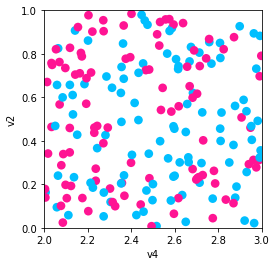
\includegraphics[width=\textwidth]{figures/code/scatter_0.png}
    \label{fig:scatter}
\end{figure}

For the scatter plot in figure~\ref{fig:scatter}, we define $Q$ as 
 \begin{equation}
    Q(\mu_{xpos}, \mu_{ypos}, \mu_{facecolor}, \mu_{s})
 \end{equation}

which we implement building on the \texttt{matplotlib.collections} API:

\begin{minted}{python}
    class Point(mcollections.Collection):
        # this is the visual fiber 
        required = {'x', 'y'}
        optional = {'facecolors', 's'} 
        def __init__(self, data, transforms, *args, **kwargs):
            """
            Parameters
            ----------
            data: sections of the fiber bundle
            transforms
            """
            super().__init__(*args, **kwargs)
            
            # check that the data you're trying to transform 
            # has a way to provide vertex data  
            assert 'vertex' in data.FB.K['tables']
            # check that you've given the required parameters
            utils.check_constraints(Point, transforms.keys())
            utils.validate_transforms(data.FB.F, transforms)
    
            self.data = data
            self.transforms = transforms
    
        def draw(self, renderer, *args, **kwargs):
            view = self.data.view('vertex') #resolve to size
    
            # call tau step
            visual = utils.convert_transforms(view, self.transforms)
               
            # assembles taus to generate idiom
            # dictionary here in place of visual(parameter) function
           
            visual['s'] = itertools.repeat(visual.get('s', 0.05))
            visual['facecolors'] = visual.get('facecolors', "C0")
            #switch out to a marker 
            self._paths = [mpath.Path.circle(center=(x,y), radius=s)  
                            for (x, y, s) 
                            in zip(visual['x'],visual['y'], visual['s'])] 
           
            self.set_facecolors(visual['facecolors'])
            super().draw(renderer, *args, **kwargs)
    \end{minted}
    
    

\end{document}